\chapter{Desarrollo}

\section{Map4rdf}
\subsection{Instalación}

Se ha optado por utilizar la máquina Virtual proporcionada en la Wiki del proyecto para minimizar la posibilidad
de incompatibilidades.

\section{GeoKettle}

Desde que se publicó ``A sustainable process and toolbox for geographical linked data generation and
publication: a case study with BTN100'' en 2019, GeoKettle ha dejado de estar soportado. La pagina oficial y de
documentación ya no están disponibles.
Un objetivo de este TFG es dar soporte GeoPackage a GeoKettle. No tiene sentido desarrollar soluciones de
``modernización'' sobre software abandonado. Por tanto, se comenzará actualizando la herramienta.

Algunas funcionalidades de GeoKettle se integraron en PDI directamente y otras desaparecieron. 
Actualmente, el soporte GIS de Pentaho está dentro de PDI Spoon y además hay algunas funcionalidades más en
 el plugin disponible en el marketplace llamado pentaho-gis-plugins. Se actualizará la primera fase a:
\textbf{``replicar la funcionalidad y las transformaciones de GeoKettle + TripleGeo en la suite PDI.''} Si es sencillo,
se considerará también dar soporte a GeoPackage.

Dado que se trata de replicar la funcionalidad anterior, se analizarán las tranformaciones realizadas por el OEG
en el repositorio de GitHub BTN100. Como se puede ver en la figura \ref{fig:spoon-missing-plugins}, partes del workflow fallan. Es lo que se pretende
solucionar.

\begin{figure}[h]
    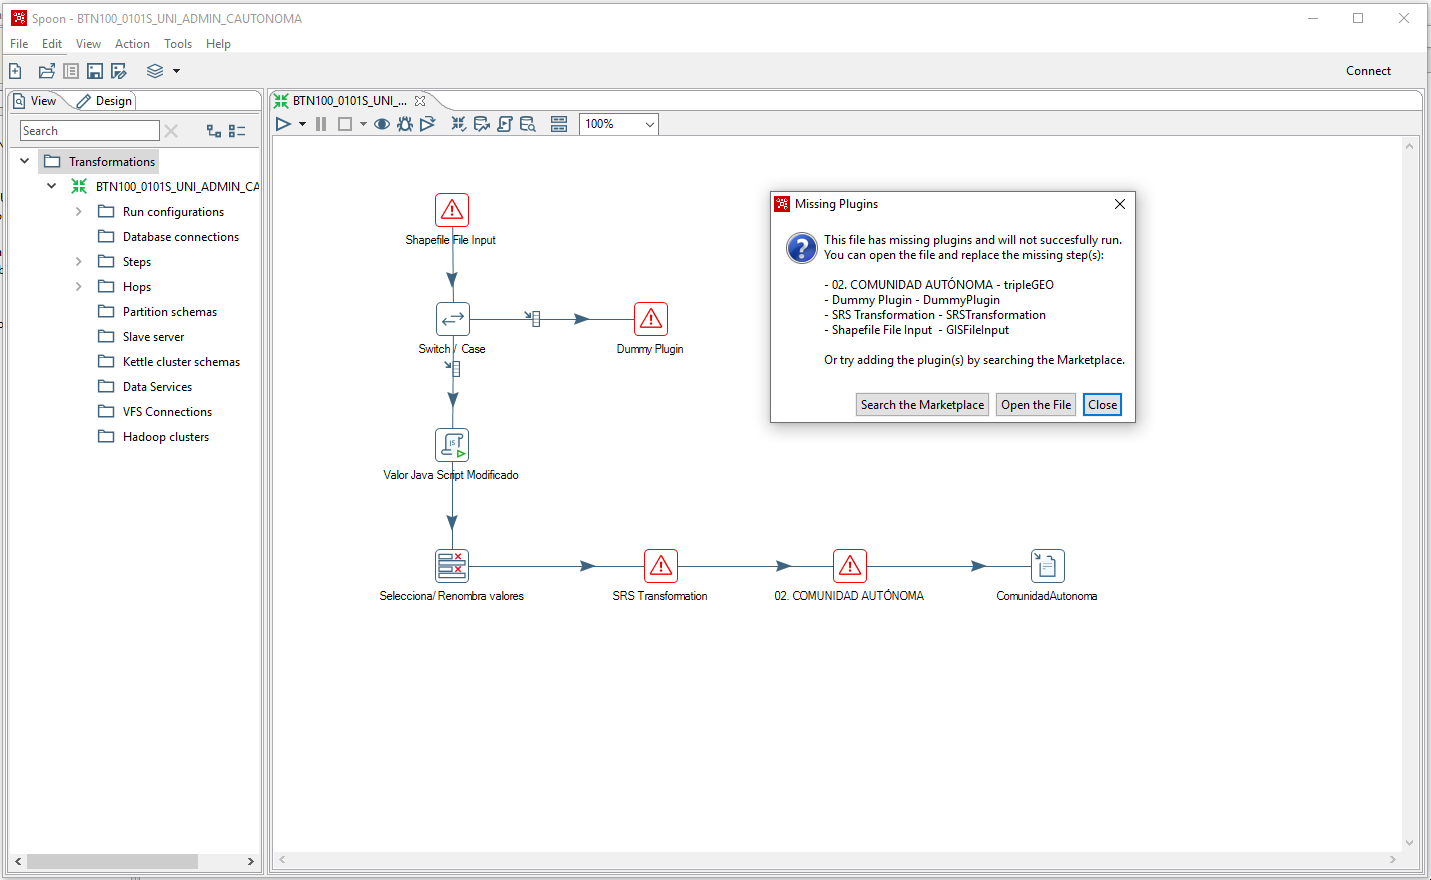
\includegraphics[width=\textwidth]{images/spoon-missing-plugins.png}
    \centering
    \caption{Workflow importado en la nueva suite}
    \label{fig:spoon-missing-plugins}
\end{figure}

